\chapter{Results and Discussion}
\label{chap:Results}
In this chapter we provide the reader with a detailed evaluation of the FIQMs and their correlation with the subjective scores collected in our subjective experiments. Since a large part of our bachelor project consisted of face image quality research, this chapter is of great importance. After conducting the experiments in Chapter \ref{chap:subjective}, we gathered a large amount of data, which we had to process (Appendix \ref{app:results}). This data will be presented in the form of statistical calculations, such as standard deviation graphs, correlation graphs, histograms and spider charts. The main goal of the chapter is to tie together the results we achieved in the objective and subjective face quality assessment, discuss them and present an in-depth look into the performance of the FIQMs relative to our collected ground truth data. The results we achieved are split into two sections. Section \ref{sec:mainExperiment} covers the results from the first subjective experiment based on the three datasets provided by Mobai, while Section \ref{sec:secondExperiment} covers the results from our own dataset. 

\section{Main Experiment}
\label{sec:mainExperiment}
In this first section the results of our first subjective experiment and the objective assessment will be presented and discussed. Both assessment categories are based on the three datasets provided by Mobai, which were described in Chapter \ref{chap:subjective}. 
%Utfylle mer her senere om hvordan seksjonen er oppbygd.


\subsection{Results of the Subjective Evaluation}
\label{sec:SubAssessment}
% Since the experiment sessions consisted of images from all datasets, the data gathered from each session had to be organized and matched with the images of the corresponding dataset. That way the ground truth data could be analyzed on the original datasets and not on the datasets used for each session.

As a first step in analyzing the subjective scores collected in our experiment, we calculated the mean opinion score (\acrshort{mos}) for the facial images in each dataset. Figure \ref{fig:MobaiHistogram} shows the histogram of the MOS results in each dataset. The score distribution for Combined passport alike and Capture from photo were quite similar which was expected given that the images in the datasets were similar in context. This was not the case in the Selfie dataset where unlike the other two datasets, images were selfies taken by the people depicted in the image. The standard deviation was calculated for every image, but also for each dataset and all datasets together. The total average standard deviation ($\overline{\sigma}$) for both experts and non-experts on all three datasets together was calculated to $\overline{\sigma} = 0.7488$. This confirmed that the participants had an equal understanding of what defined a good or bad facial image. The instruction manual likely affected the quality perception of the participants as anticipated. Given that we were collecting ground truth data, it was expected that the deviation should be low.   

\begin{figure}[h]
    \centering
    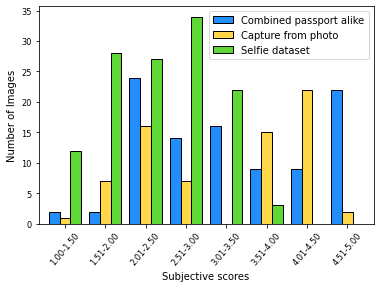
\includegraphics[width=0.65\textwidth]{figures/MobaiDS_Histogram.png}
    \caption{Histogram of MOS values calculated  for the images in each dataset. There is a clear difference between the quality of the Selfie dataset and the two others.}
    \label{fig:MobaiHistogram}
\end{figure}

Figure \ref{fig:MobaiDS} depicts three line plots of the standard deviation of the subjective scores on all images in each dataset. The plots show the subjective score distribution and they take into consideration the total standard deviation and the deviation of each participant group. Whenever the three lines have a low spread between each other it indicates that the deviation of the participant groups were similar. The lower the deviation the more the majority of the participants agreed upon a similar score. This was especially apparent in the Combined passport alike dataset (Figure \ref{fig:combinedpassportalikeSD}) which also generated the lowest total standard deviation of $\sigma = 0.6707$. The two remaining datasets (Figure \ref{fig:capturefromphotoSD} and \ref{fig:selfiedatasetSD}) received a similar total standard deviation of $\sigma = 0.7891$ and $\sigma = 0.7872$ respectively. Some images had greater variety than others. The Selfie dataset contained some of those, but all in all the general participants rated images alike. Even between the experts and non-experts, the evaluation was more or less equal. In fact non-experts had a slightly better standard deviation of $\sigma = 0.6908$, than the experts of $\sigma = 0.7608$ on the three datasets. 

Four images were chosen and previewed from each dataset. The first plot, Figure \ref{fig:combinedpassportalikeSD}, which showcases Combined passport alike, the first and second images would be considered excellent facial images. The experts rated these images very similarly which is apparent by the low deviation scores. The spread amongst non-experts were greater with deviations around 1.0. The two remaining images were of lower face quality, but the deviations were not affected by that.  


\begin{figure}[H]
 \centering 
    \subfloat
        {\hspace{1cm}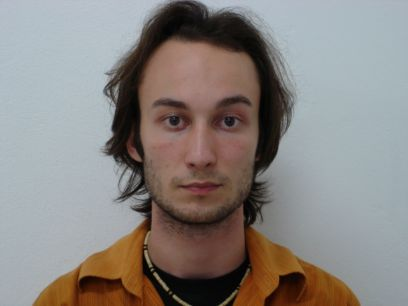
\includegraphics[scale = 0.1]{figures/042.jpg}\hspace{1.3cm}}
    \subfloat
        {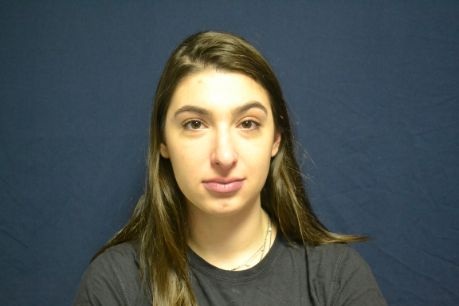
\includegraphics[scale = 0.1]{figures/132.jpg}\hspace{0.3cm}}
    \subfloat
        {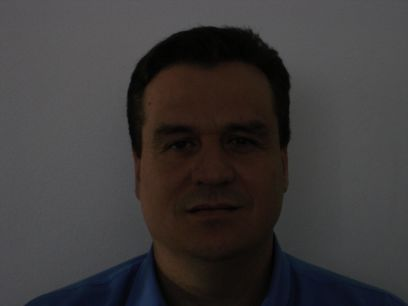
\includegraphics[scale = 0.1]{figures/145.jpg}\hspace{1.1cm}}
    \subfloat
        {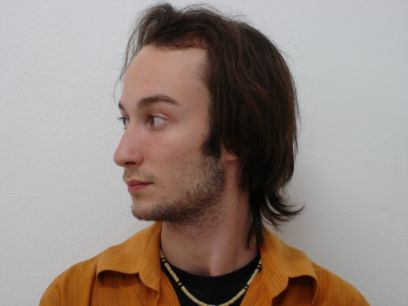
\includegraphics[scale = 0.1]{figures/234.jpg}\hspace{0.3cm}}
    \quad
    \addtocounter{subfigure}{-4}
    \subfloat[Combined passport alike dataset]
        {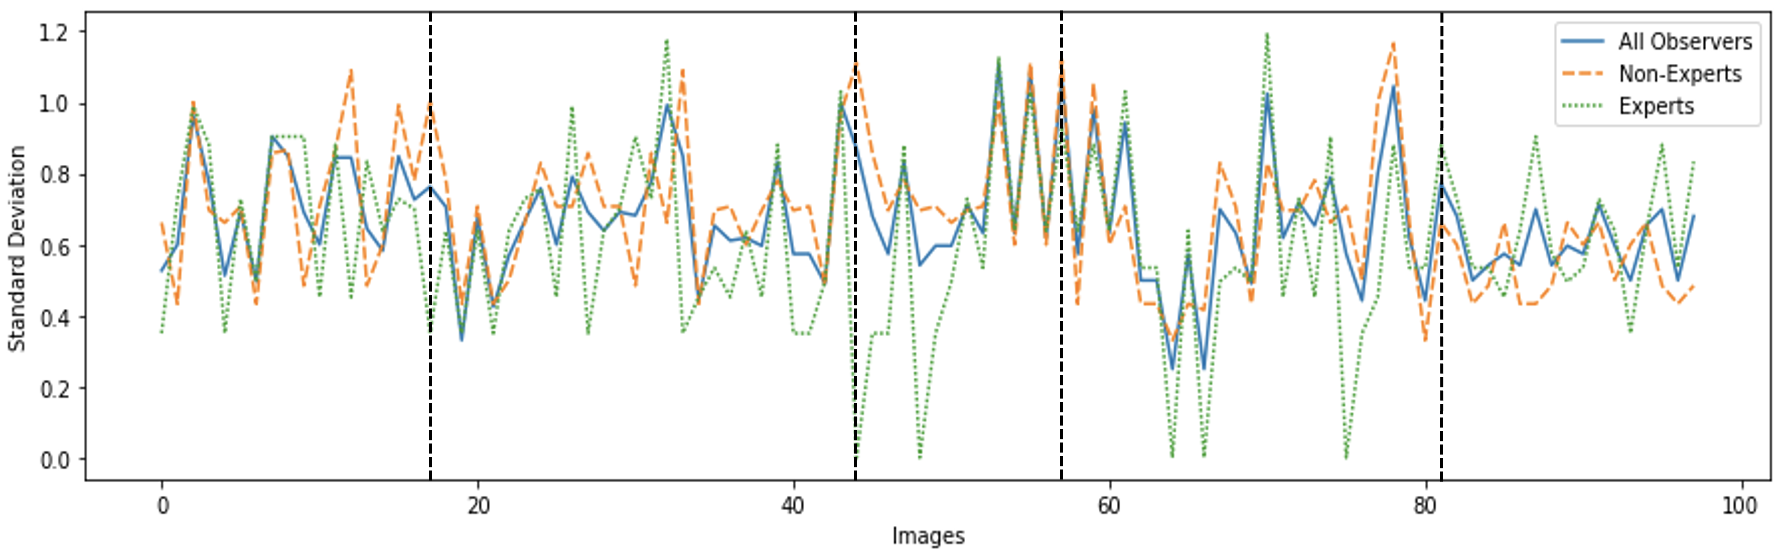
\includegraphics[width=1.0\textwidth]{figures/STD.png}\label{fig:combinedpassportalikeSD}}
        \quad
        \vspace{1cm}
    
    \subfloat
        {\hspace{0.7cm}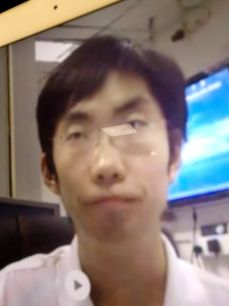
\includegraphics[scale = 0.12]{figures/004.jpg}\hspace{1.5cm}}
    \subfloat
        {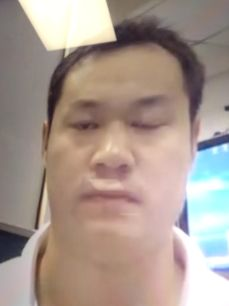
\includegraphics[scale = 0.12]{figures/101.jpg}\hspace{4.3cm}}
    \subfloat
        {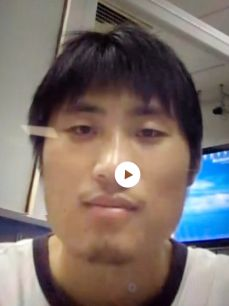
\includegraphics[scale = 0.12]{figures/198.jpg}\hspace{0.1cm}}
    \subfloat
        {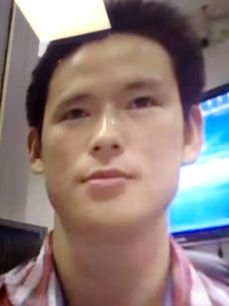
\includegraphics[scale = 0.12]{figures/204.jpg}\hspace{2.4cm}}
    \quad
    \addtocounter{subfigure}{-4}
    \subfloat[Capture from photo dataset]
         {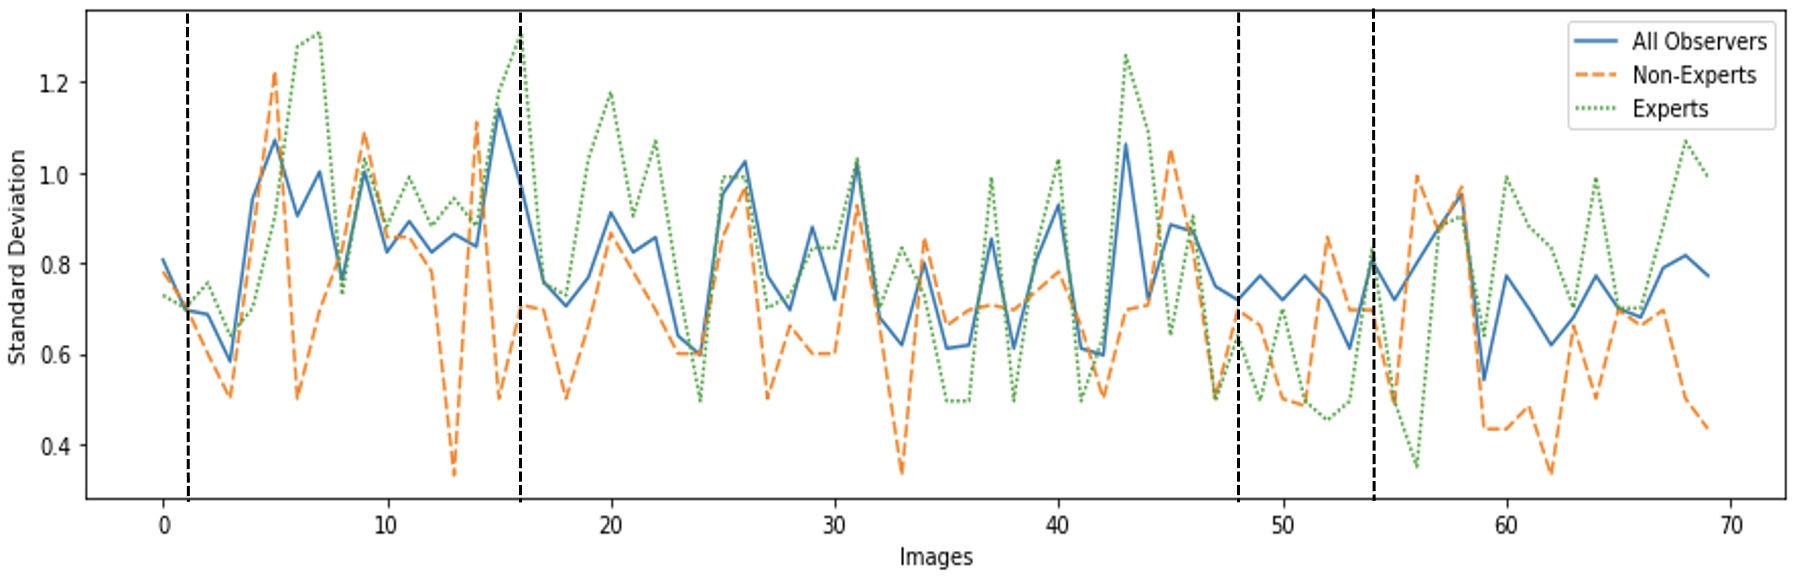
\includegraphics[width=1.0\textwidth]{figures/STD2.png}\label{fig:capturefromphotoSD}}
        \quad
        \vspace{1cm}
        
    \subfloat
        {\hspace{1.7cm}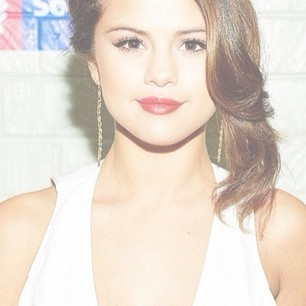
\includegraphics[scale = 0.1]{figures/086.jpg}\hspace{0.2cm}}
    \subfloat
        {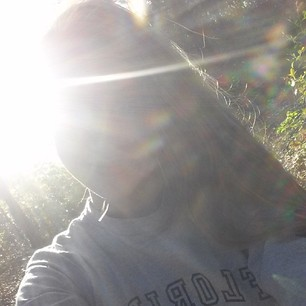
\includegraphics[scale = 0.1]{figures/098.jpg}\hspace{1.8cm}}
    \subfloat
        {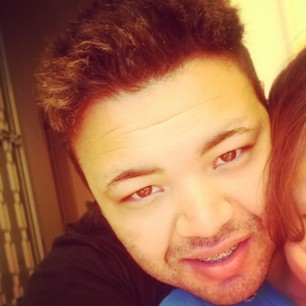
\includegraphics[scale = 0.1]{figures/187.jpg}\hspace{1.6cm}}
    \subfloat
        {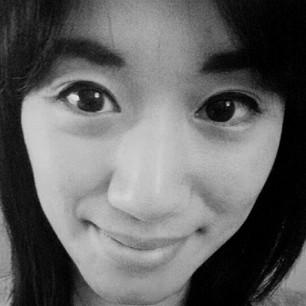
\includegraphics[scale = 0.1]{figures/271.jpg}\hspace{1cm}}
    \quad
    \addtocounter{subfigure}{-4}
    \subfloat[Selfie dataset]
         {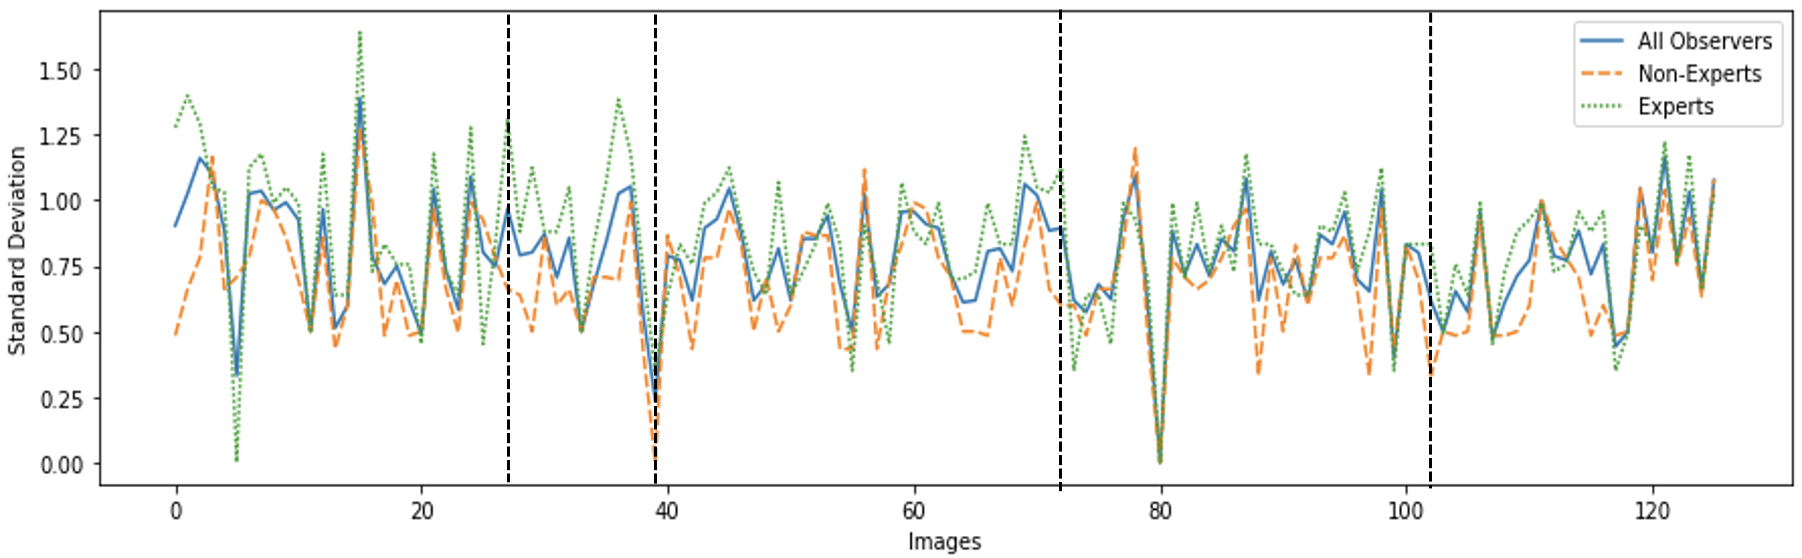
\includegraphics[width=1.0\textwidth]{figures/STD3.png}\label{fig:selfiedatasetSD}}
     \caption{Standard deviation values of the subjective scores given to each image in the three datasets. Sample images from each dataset are shown as examples.}
     \label{fig:MobaiDS}
\end{figure}

The four next facial images of Capture from photo in Figure \ref{fig:capturefromphotoSD} shows an overall equal standard deviation between the non-experts and experts. However, the second image had notable differences in the subjective scores between non-experts and experts. The standard deviation amongst experts were close to 1.2, which was the highest of the dataset. The great distribution of scores was likely due to the nature of the facial image. On one side the face is visible, but on the other side the image is taken from a computer screen which has heavily reduced the appearance of the face. This also applies to the last two images, however the standard deviation was lower and more even between the experts and non-experts.

The last four previewed facial images belong to the Selfie dataset (Figure \ref{fig:selfiedatasetSD}). The first image had an total deviation of 0.90. It was highly likely that the deviation of 0.90 was because the face was off-centered and not fully shown, which was the case for a large portion of the Selfie dataset images. However the second image had considerably lower standard deviation values. The face was barely visible which both participant groups assessed similarly. The scores of the experts on the last two images were more spread than the non-experts. 

\subsection{Evaluating the Performance of FIQMs}
The FIQMs presented in Chapter \ref{chap:FQA} use different approaches to predict the perceived face quality. Their predicted perception of quality is supposed to correlate with human assessment, which is the whole purpose of FIQMs. The objective predictions produced by the FIQMs were measured against human assessment to evaluate the accuracy of the proposed approaches. This evaluation was carried out by calculating the correlation coefficients. The sample Pearson correlation coefficient ($r$) was calculated as: 
\begin{equation}
    {\displaystyle r={\frac {\sum _{i=1}^{n}(x_{i}-{\bar {x}})(y_{i}-{\bar {y}})}{{\sqrt {\sum _{i=1}^{n}(x_{i}-{\bar {x}})^{2}}}{\sqrt {\sum _{i=1}^{n}(y_{i}-{\bar {y}})^{2}}}}}}
\end{equation}
where $n$ is the sample size, $x_{i}$ and $y_{i}$ denotes the individual sample scores from the objective and the subjective assessment respectively, while ${\bar {x}}={\frac {1}{n}}\sum _{i=1}^{n}x_{i}$ and ${\bar {y}}={\frac {1}{n}}\sum _{i=1}^{n}y_{i}$ represents the sample means from the objective and the subjective scores. Another type of correlation coefficient, the Spearman rank correlation coefficient ($\rho$) \cite{wiki:spearman} was also calculated because it does not assume that both variables are normally distributed.

The subjective scores were normalized in order to achieve the same ranking scale when being compared with the objective scores. Our subjective experiment initially had a categorical judgment with a scale from one to five, which was converted to scores between zero and one. It is easy to think that the MOS for each image should be divided by the number of score alternatives in the subjective experiment, which in this case was five. However it is worth noting that had we only divided the subjective scores by five, the lowest subjective scores achievable would be 0.2. This means that the FIQMs could provide scores from zero to one, while the subjective scores were from 0.2 to one. Dividing by five would therefore provide us with an uneven scoring scale where a score of five equals 100\% while the lowest score of one equals 20\% instead of 0\%. We needed a five-point scale that would increment the score alternatives with 25\% starting from 0\%. To properly convert a five-point scale to percentages we used the following equation (\ref{eqn:MOS}) on every image:

\begin{equation}
    MOS_{Normalized} = \frac{MOS - 1}{4}
    \label{eqn:MOS}
\end{equation}

\subsubsection{ISO Metrics}
\begin{figure}[h]
\centering
    \subfloat[Combined passport alike]
        {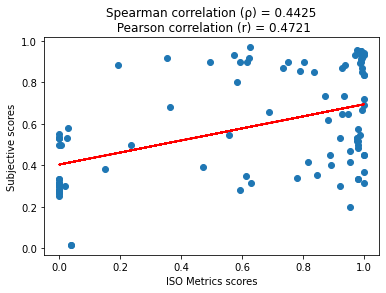
\includegraphics[scale = 0.31]{figures/ISO_Subjective1.png}\label{fig:iso_SUB1}}
    \subfloat[Capture from photo]
        {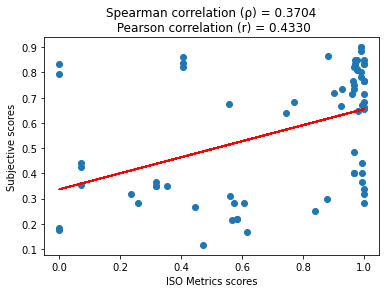
\includegraphics[scale = 0.31]{figures/ISO_Subjective2.png}\label{fig:iso_SUB2}}
    \subfloat[Selfie dataset]
        {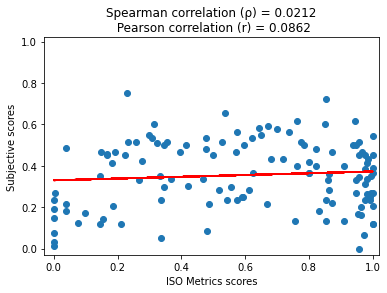
\includegraphics[scale = 0.31]{figures/ISO_Subjective3.png}\label{fig:iso_SUB3}}
    \caption{2D scatter plots of the objective and subjective scores on the three datasets with objective scores along the x-axis and the subjective scores along the y-axis. The Spearman and Pearson correlation coefficients are shown above each plot.}
    \label{fig:corrISOsvsSub}
\end{figure}
\noindent 
As a first step in analyzing the performance of FIQMs, we calculate the correlation between the subjective scores and the objective scores calculated by the metrics. Figure \ref{fig:corrISOsvsSub} provides different plots of subjective against objective scores for the three introduced datasets. The correlation coefficients on Combined passport alike and Capture from photo were just shy of 0.5 which indicated a low to moderate association, whereas the correlation on the Selfie dataset was non-existent. The performance of ISO Metrics was clearly worse on the Selfie dataset relative to the two others. The FIQM was challenged by the dataset which was not surprising given that the images were of mediocre face quality which ISO Metrics often tends to over evaluate. In other words ISO Metrics was not suited for the Selfie dataset.  

\subsubsection{FaceQnet}
\begin{figure}[h]
\centering
    \subfloat[Combined passport alike]
        {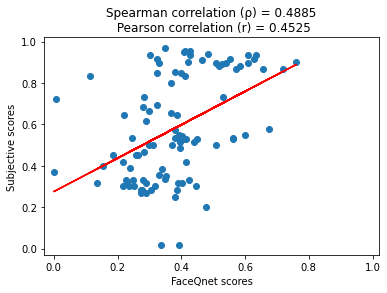
\includegraphics[scale = 0.31]{figures/FaceQNet_Subjective1.png}\label{fig:face_SUB1}}
    \subfloat[Capture from photo]
        {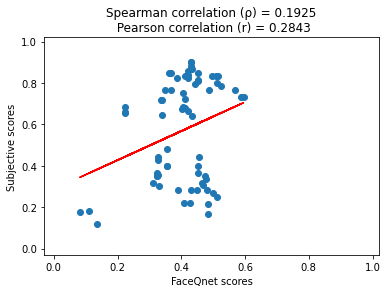
\includegraphics[scale = 0.31]{figures/FaceQNet_Subjective2.png}\label{fig:face_SUB2}}
    \subfloat[Selfie dataset]
        {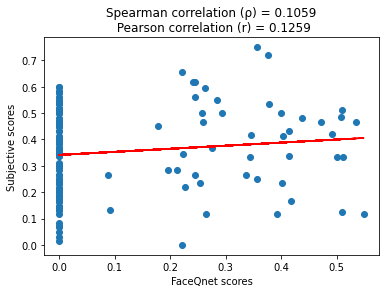
\includegraphics[scale = 0.31]{figures/FaceQNet_Subjective3.png}\label{fig:face_SUB3}}
    \caption{2D scatter plots of the objective and subjective scores on the three datasets with objective scores along the x-axis and the subjective scores along the y-axis. The Spearman and Pearson correlation coefficients are shown above each plot.}
    \label{fig:corrFACEQNETsvsSub}
\end{figure}
\noindent
The correlation between FaceQnet and the subjective scores regressed with each dataset the same way as ISO Metrics and the subjective scores did, shown in Figure \ref{fig:corrFACEQNETsvsSub}. The performance of the two FIQMs was comparable on all the datasets. Combined passport alike achieved the highest correlation of the datasets, with Spearman and Pearson values similar to the ones in Figure \ref{fig:iso_SUB1}. Like ISO Metrics, the performance of FaceQnet on Capture from photo was worse than Combined passport alike, but this time FaceQnet performed slightly worse than ISO Metrics. The performance on the Selfie dataset was even worse with a non-existing negligible correlation. A large part of the Selfie dataset images were rated zero. The facial images rated zero were mostly because the cropping part of FaceQnet failed. This happened when the cropping part failed to detect the face of the images. The images were therefore manually provided a score of zero. In other words, FaceQnet is not a suitable FIQM for the Selfie dataset. 

\subsubsection{Could We Use Different FIQMs Simultaneously?}
An interesting idea the team came up with, was if the correlation between the FIQMs and the subjective scores could be improved if a weighted average of the two FIQMs were used as the final FIQM. As a first step in such an approach, we simply gave the same weight to both FIQMs and tested the idea on the Combined passport alike and Capture from photo datasets. Since FaceQnet did not work for over 50\% of the images in the Selfie dataset, we found no reason to test this approach on that dataset. 

Figure \ref{fig:corrAVGvsSub} shows the correlation coefficients and the linear regression line calculated on the two datasets. The plot depicted in Figure \ref{fig:avg_SUB1} shows the highest correlation coefficients we ever achieved during our experiments. The $r$-value of 0.6045 and the $\rho$-value of 0.5942 were considerably higher than the correlation coefficients of the FIQMs individually. A value around 0.6 would indicate a moderate to strong correlation between the two data types. Even Capture from photo showed an increase in the correlation value. Initially, ISO Metrics performed better on the dataset than FaceQnet, but after the weighted average approach, the combined scores performed slightly better than ISO Metrics. Nevertheless, the correlation was still considered low to moderate. 
\begin{figure}[h]
\centering
    \subfloat[Combined passport alike]
        {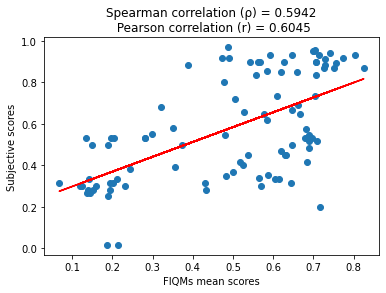
\includegraphics[scale = 0.45]{figures/FIQMAVGSubjective1.png}\label{fig:avg_SUB1}}
    \subfloat[Capture from photo]
        {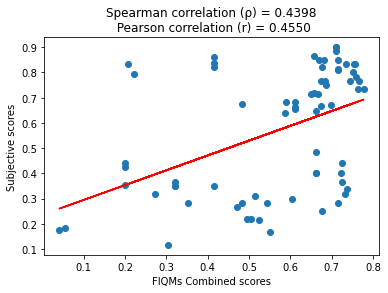
\includegraphics[scale = 0.45]{figures/FIQMAVGSubjective2.png}\label{fig:avg_SUB2}}
    \caption{2D scatter plots of the scores provided by using a weighted average of the FIQMs (with the same weight) on Combined passport alike and Capture from photo. The average FIQMs scores are displayed along the x-axis and subjective scores along the y-axis. The Spearman and Pearson correlation coefficients are presented above the plots.}
    \label{fig:corrAVGvsSub}
\end{figure}

\subsubsection{Error Method}
Plotting the results of the FIQMs against the subjective scores was not enough to assess the performance of the FIQMs on the datasets. Although the correlation coefficients on the datasets mostly were below 0.5 and indicated low to moderate correlation, error methods such as Root Mean Square Error (\acrshort{rmse}) can be used to track both the efficiency and accuracy of our FIQMs. The RMSE values were calculated by the following general formula: 
\begin{equation}
    RMSE = \sqrt{\frac{1}{N}\sum _{i=1}^{N}(Predicted_{i} - Actual_{i})^2}
    \label{eqn:RMSE}
\end{equation}
%
In Equation \ref{eqn:RMSE} $N$ corresponds to the number of samples, and in our case these were images. The predicted values denoted the objective scores by the FIQMs while the actual values were the corresponding subjective scores. This calculation gave us the standard deviation of the prediction errors. In other words, RMSE measured how far from the linear regression line the predicted values were. The closer to zero the scores were, the better the FIQMs predicted the right scores.

\begin{table}[h]
\caption{The calculated RMSE values of the FIQMs on the datasets relative to the subjective scores. The RMSE value was not calculated for the Selfie dataset with a weighted average of the FIQMs. The `X' symbolises this.}
\resizebox{\textwidth}{!}{%
\begin{tabular}{|
>{\columncolor[HTML]{EFEFEF}}c |
>{\columncolor[HTML]{FFFFFF}}c |
>{\columncolor[HTML]{FFFFFF}}c |
>{\columncolor[HTML]{FFFFFF}}c |}
\hline
\multicolumn{1}{|c|}{\cellcolor[HTML]{C0C0C0}\textbf{RMSE values}} &
  \multicolumn{1}{c|}{\cellcolor[HTML]{EFEFEF}ISO Metrics} &
  \cellcolor[HTML]{EFEFEF}FaceQnet &
  \multicolumn{1}{c|}{\cellcolor[HTML]{EFEFEF}FIQMs Weighted AVG} \\ \hline
Combined passport alike & 0.3675 & 0.3031 & 0.2262 \\ \hline
Capture from photo      & 0.3551 & 0.2887 & 0.2309 \\ \hline
Selfie dataset          & 0.4342 & 0.3253 & X \\ \hline
\end{tabular}%
}
\label{tab:RMSE}
\end{table}
%\noindent
The highest correlation coefficient, without using the weighted average approach on the FIQMs, was achieved on the Combined passport alike dataset with ISO Metrics as shown in Figure \ref{fig:iso_SUB1}. Although the correlation was around 0.5, the RMSE value was around 0.36, shown in Table \ref{tab:RMSE}. This meant that on average, the perceived quality predicted by ISO Metrics was off by $\pm$0.36 points compared to the actual subjective scores. Since our scale was from zero to one, 0.36 points off equaled an error of $\pm$36\% which was remarkably high. Even worse was the RMSE value on the Selfie dataset with ISO Metrics with a staggering error of 43\%. Despite having a lower correlation with the subjective scores on average, FaceQnet outperformed ISO Metrics on all datasets with its RMSE values. On average, FaceQnet´s errors were 0.8 points lower than ISO Metrics which equaled an error decrease of 20\%. 

The interesting results were those of the weighted average FIQMs. They ach-
ieved considerably better values than the FIQMs individually. Although an error of $\pm$0.22 and $\pm$0.23 in our case would be considered mediocre, the decrease could not be overlooked. Weighted average FIQMs had a decreased error rate of $\pm$0.14 points on Combined passport alike and $\pm$0.08, relative to ISO Metrics and FaceQnet. This equaled a decrease of 38.5\% and 25.4\% respectively. The accuracy of weighted average FIQMs was similar on the Capture from photo dataset. 

\subsection{Significance of Our Results}
Our results without any kind of validation were of little value. A validation had to be done in order to conclude whether our results were statistical significant. We had to be confident that our results could be replicated and that they did not occur by coincidence. 

The plots depicted in Figure \ref{fig:corrISOsvsSub} and Figure \ref{fig:corrFACEQNETsvsSub} showed for the most part, except for the Selfie dataset, a low to moderate correlation between the objective and subjective scores. The correlation coefficients were calculated with a 95\% confidence interval, which gave us a significance level of 0.05. The p-values of the correlation coefficients were calculated and the lower the p-value the more statistical significant our results were. Anything above a value of $p = 0.05$ was considered insignificant, because it meant that the likelihood of an uncorrelated system providing those exact coefficients randomly would be 5\%. 

Table \ref{tab:corrcoeff} show only the correlation coefficients that were considered statistically significant, i.e. we were 95\% confident the correlation coefficients did not occur by coincidence. The coefficients were replaced by an `X' symbol where the p-values were greater than the significance level and should therefore be taken with a grain of salt. All results regarding whether the FIQMs were correlated with the subjective scores on the Selfie dataset were confirmed to be uncorrelated with the high p-values. With a combination of high p-values and low correlation coefficients, it is highly likely that the objective and subjective scores were uncorrelated. The results gathered from the remaining datasets were within the significance level and were considered accurate.  


\begin{table}[h]
\caption{All correlation coefficients on the three datasets between ISO Metrics, FaceQnet, FIQMs Weighted AVG and the subjective scores. The `X'-symbol indicated the correlation coefficients that had a p-value higher than 0.05 and were therefore ignored. The coefficients were not calculated where the `-' symbol is placed.}
\resizebox{\textwidth}{!}{%
\begin{tabular}{l|
>{\columncolor[HTML]{FFFFFF}}c |
>{\columncolor[HTML]{FFFFFF}}c |
>{\columncolor[HTML]{FFFFFF}}c |
>{\columncolor[HTML]{FFFFFF}}c |
>{\columncolor[HTML]{FFFFFF}}c |
>{\columncolor[HTML]{FFFFFF}}c |}
\cline{2-7}
 &
  \multicolumn{2}{c|}{\cellcolor[HTML]{C0C0C0}\textbf{ISO Metrics}} &
  \multicolumn{2}{c|}{\cellcolor[HTML]{C0C0C0}\textbf{FaceQnet}} &
  \multicolumn{2}{c|}{\cellcolor[HTML]{C0C0C0}\textbf{FIQMs Weighted AVG}} \\ \cline{2-7} 
\textbf{} &
  Spearman $\rho$ &
  Pearson $r$ &
  Spearman $\rho$ &
  Pearson $r$ &
  Spearman $\rho$ &
  Person $r$ \\ \hline
\multicolumn{1}{|l|}{\cellcolor[HTML]{C0C0C0}Combined passport alike} &
  0.4425 &
  0.4721 &
  0.4885 &
  0.4525 &
  0.5942 &
  0.6045 \\ \hline
\multicolumn{1}{|l|}{\cellcolor[HTML]{C0C0C0}Capture from photo} &
  0.3704 &
  0.4330 &
  X &
  0.2843 &
  0.4398 &
  0.4550 \\ \hline
\multicolumn{1}{|l|}{\cellcolor[HTML]{C0C0C0}Selfie dataset} &
  X &
  X &
  X &
  X &
  - &
  - \\ \hline
\end{tabular}%
}
\label{tab:corrcoeff}
\end{table}
%\noindent


\section{Second Experiment}
\label{sec:secondExperiment}
This section is about the second experiment we conducted based on our own NFC dataset of 450 images, and the results we achieved. A key goal the team considered was having the NFC dataset consist of varying face quality to achieve a balanced dataset. A histogram of the MOS values calculated in the second subjective experiment on the NFC dataset is depicted in Figure \ref{fig:NFCHistogram}. One can see how the different quality categories are represented to an acceptable level. Images of specific quality were not over represented relative to the other quality categories and there exist a nice distribution in the dataset with images of varying quality which was the goal of the group. 

\begin{figure}[h]
    \centering
    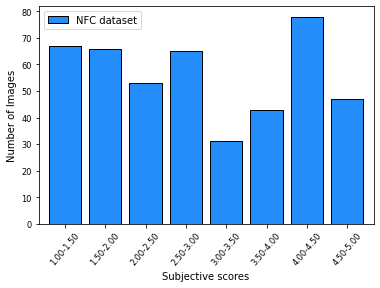
\includegraphics[width=0.5\textwidth]{figures/NFC_Histogram.png}
    \caption{Histogram of the subjective scores on the NFC dataset.}
    \label{fig:NFCHistogram}
\end{figure}

\subsection{Results of the Subjective Evaluation}
The MOS of each image was calculated as we did in the first subjective experiment in Section \ref{sec:SubAssessment}. The subjective scores of the NFC dataset provided by the participants correlated closely. The average standard deviation of the subjective scores was calculated to be $\overline{\sigma} = 0.53$ which was substantially lower than those of the datasets in the first subjective experiment mentioned in Section \ref{sec:SubAssessment}. This time the experiment was not split into several sessions to prevent fatigue even though it consisted of several times the facial images of the first subjective experiment. With that in mind the average standard deviation was lower, which goes to show how the subjective experiment aspects mentioned in Section \ref{sec:SubjectiveAspects} mattered to a lesser degree since we were collecting ground truth data. Provided that six subjects participated in the subjective experiment and only two of those were experts we found no reason to compare the standard deviations between those types of participants.


\subsection{Results of the Objective Evaluation}
An important metric we voluntary wanted to measure was how the FIQMs performed on distorted images relative to their corresponding undistorted ones. This was tested on a subset of the NFC dataset which consisted of the 200 distorted images and their 50 corresponding original images. In order to assess how the FIQMs performed we first had to analyze how the subjective scores were distributed. A histogram of the MOS values for different types of distortions are shown in Figure \ref{fig:NFC2HistogramSUB}. From Figure \ref{fig:NFC2HistogramSUB} it is clear that the distortions we added to the images did not have a considerable affect on the subjective scores. It is interesting to investigate how such distortions can affect the performance of FIQMs.

\begin{figure}[h]
    \centering
    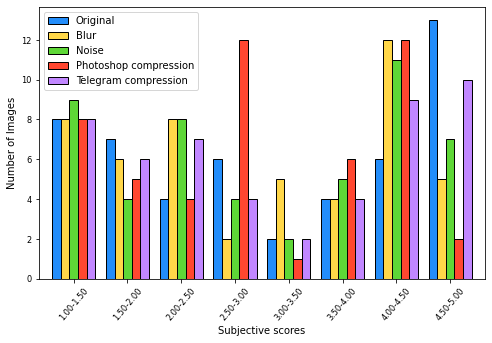
\includegraphics[width=0.5\textwidth]{figures/NFC_HistogramSUB.png}
    \caption{Histogram of the subjective scores of the original images and their corresponding distorted images in the NFC dataset.}
    \label{fig:NFC2HistogramSUB}
\end{figure}

\begin{figure}[h]
\centering
    \subfloat[ISO Metrics scores]
        {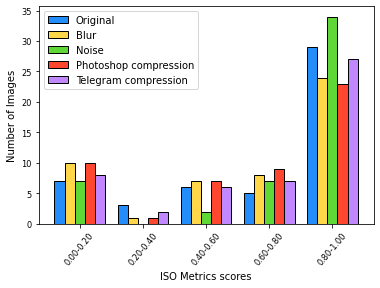
\includegraphics[ width=0.47\textwidth]{figures/NFC_HistogramISO.png}\label{fig:HistogramISO}}
    \subfloat[FaceQnet scores]
        {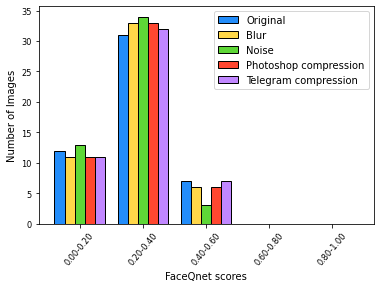
\includegraphics[width=0.47\textwidth]{figures/NFC_HistogramFaceQnet.png}\label{fig:HistogramFACE}}
    \caption{Histogram of the objective scores of the original images and their corresponding distorted images in the NFC dataset.}
    \label{fig:NFC2Histogram}
\end{figure}

Figure \ref{fig:NFC2Histogram} showcases how the FIQMs performed on the original and distorted images. Even though the scores provided vastly differed from the subjective scores, one can see how the objective scores highly correlated between the different distortions. Among the FIQMs, FaceQnet had an overall better performance on the types of distortions we added relative to ISO Metrics. Its scores correlated close to perfect which is shown in Figure \ref{fig:NFCFaceCorr}. Three out of four distortions had correlation coefficients above 0.8, which is considered a very strong positive correlation. Only the Telegram compression on FaceQnet performed slightly worse with a moderate to high correlation. ISO Metrics performed likewise, however the scores were more spread as shown in Figure \ref{fig:HistogramISO}. The scores of facial images with noise differed noticeably from its original ones. Facial images with noise also had a significantly lower correlation than the other distortions, shown in Figure \ref{fig:NFCISOCorr}. The FIQM struggled with facial images with noise which is clear by the moderate correlation coefficients close to 0.5, relative to the other distortions which are considered strongly correlated. Not only did the correlation coefficients confirm that FaceQnet performed better on the distortions, but the FIQM had considerably lower RMSE values on $\frac{3}{4}$ distortions than ISO Metrics. Only by looking at the RMSE values mentioned above each plot depicted in Figure \ref{fig:NFCFaceCorr} and Figure \ref{fig:NFCISOCorr}, it is clear that ISO Metrics is less consistent than FaceQnet when assessing distorted images. 

\begin{figure}[H]
\centering
    \subfloat
        {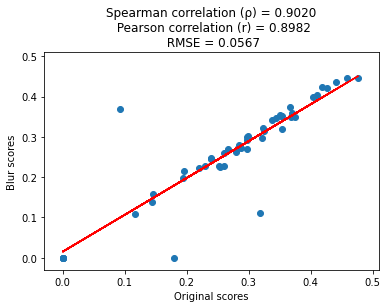
\includegraphics[width=0.37\textwidth]{figures/FaceQnetBlur.png}}
    \subfloat
        {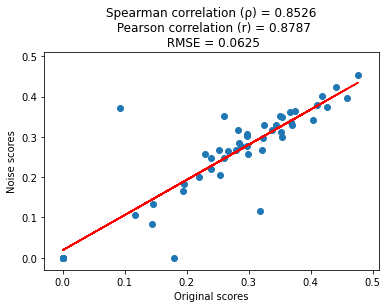
\includegraphics[width=0.37\textwidth]{figures/FaceQnetNoise.png}}
        \quad
    \subfloat
        {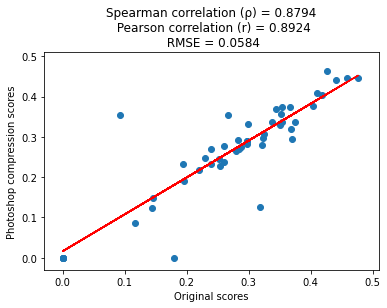
\includegraphics[width=0.37\textwidth]{figures/FaceQnetPhotoshop.png}}
    \subfloat
        {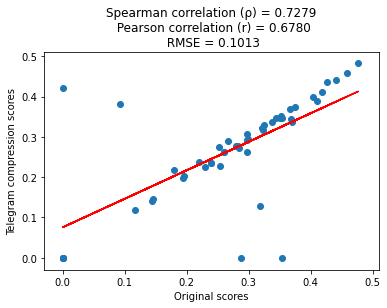
\includegraphics[width=0.37\textwidth]{figures/FaceQnetTelegram.png}}
    \caption{2D scatter plots of FaceQnet scores on the original images along the x-axis and the distorted images along the y-axis. All correlation coefficients are given with a 95\% confidence interval. RMSE values are included above the plots.}
    \label{fig:NFCFaceCorr}
\end{figure}

\begin{figure}[h]
\centering
    \subfloat
        {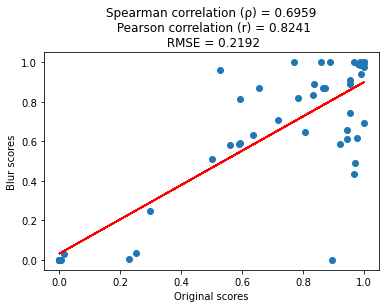
\includegraphics[width=0.365\textwidth]{figures/ISOBlur.png}}
    \subfloat
        {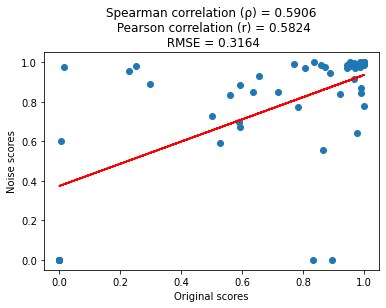
\includegraphics[width=0.365\textwidth]{figures/ISONoise.png}}
        \quad
    \subfloat
        {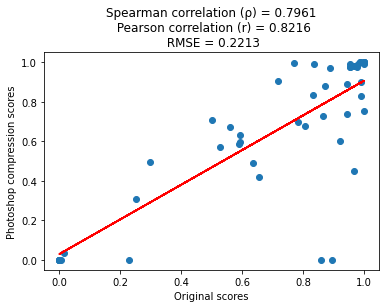
\includegraphics[ width=0.365\textwidth]{figures/ISOPhotoshop.png}}
    \subfloat
        {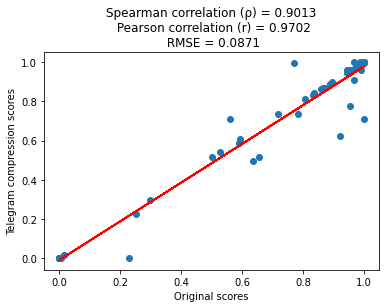
\includegraphics[width=0.365\textwidth]{figures/ISOTelegram.png}}
    \caption{2D scatter plots of ISO Metrics scores on the original images along the x-axis and the distorted images along the y-axis. All correlation coefficients are given with a 95\% confidence interval. RMSE values are included above the plots.}
    \label{fig:NFCISOCorr}
\end{figure}

\subsection{Evaluating the Performance of FIQMs}
The correlation between the FIQMs and the collected subjective scores was calculated and plotted in Figure \ref{fig:ourDS1corr}. A 0.05 significance level was used when calculating the correlation coefficients. The coefficients ranged between 0.32 to 0.42 which meant there was a weak association between the objective and subjective scores. Using a weighted average of the two FIQMs did not show a significant difference. There were no clear difference between the performance of either FIQM on our dataset. Even though the correlation was weak, the result were not entirely negative. Our dataset was supposed to challenge the FIQMs by introducing new measures they had not been exposed to or created to assess, which was the case. 

\begin{figure}[H]
\centering
    \subfloat[ISO Metrics]
        {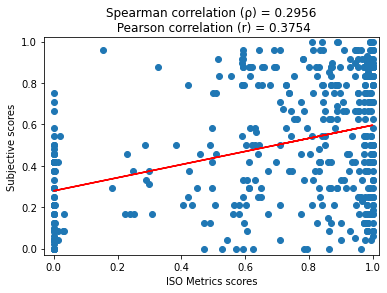
\includegraphics[scale = 0.31]{figures/NFCISOSUB.png}\label{fig:our1_ISO}}
    \subfloat[FaceQnet]
        {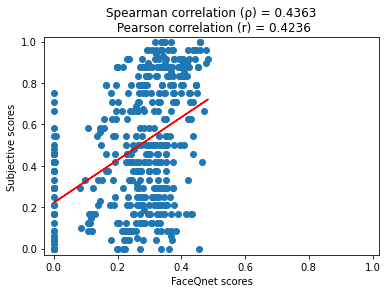
\includegraphics[scale = 0.31]{figures/NFCFACESUB.png}\label{fig:our1_FACE}}
    \subfloat[FIQMs Weighted AVG]
        {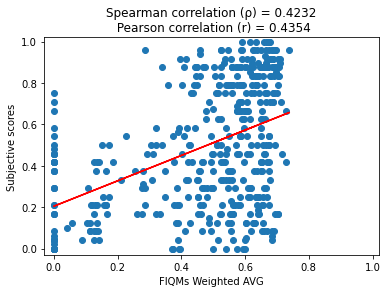
\includegraphics[scale = 0.31]{figures/NFCWeightedAVG.png}\label{fig:our1_AVG}}
    \caption{2D scatter plots of the scores on the NFC dataset with objective scores along the x-axis and subjective scores along the y-axis. The Spearman and Pearson correlation coefficients are shown above the plots.}
    \label{fig:ourDS1corr}
\end{figure}

\subsubsection{Score Distribution on Distorted Images} 

The spider chart in Figure \ref{fig:spiderMask} takes a closer look into how the FIQMs reacted to the different face mask usages. The subjective scores for 0940.jpg and 1133.jpg were lower than the two other face mask images because the face is more covered and therefore less visible. ISO Metrics did not react to that whatsoever, but Face-Qnet did provide slightly lower scores, but the change was very minor. Regarding the spider plot of the oblique angled images depicted in Figure \ref{fig:spiderTilted}, both FIQMs provided lower scores than the subjective, but the ISO Metrics scores were consistent where as FaceQnet had larger differences between the facial images.

The two spider plots depicted in Figure \ref{fig:SpiderDist1} and Figure \ref{fig:spiderDist2} are used to show the score distribution of the previewed distorted facial images. On image 0329.jpg in Figure \ref{fig:SpiderDist1} we can see how ISO Metrics predicted equal scores, but the facial image with noise had a major effect on the score. This is consistent with the histogram in Figure \ref{fig:HistogramISO}. Even the Photoshop compression received double the score of its original image. FaceQnet had an overall more consistent quality perception close to the subjective scores. Image 0718.jpg in Figure \ref{fig:spiderDist2} again showed how FaceQnet was not affected by adding any of our distortions. The plot reinforces the claim that the distribution of objective scores on distorted images were negligible with FaceQnet, which is shown in Figure \ref{fig:HistogramFACE}. The FaceQnet scores were quality wise closely related to the subjective scores, whereas the quality perception by ISO Metrics was off. This time, the FIQM gave much more consistent scores with no large spikes, which goes to show its inconsistency.


\begin{figure}[H]
\centering
    \subfloat[Different use of face masks.]
        {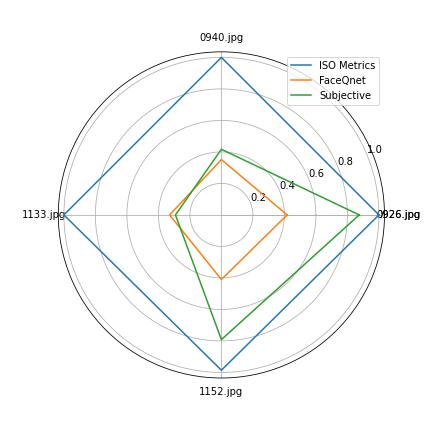
\includegraphics[width=0.42\textwidth]{figures/SpiderMask.png}} \\
    \subfloat[0926.jpg]
        {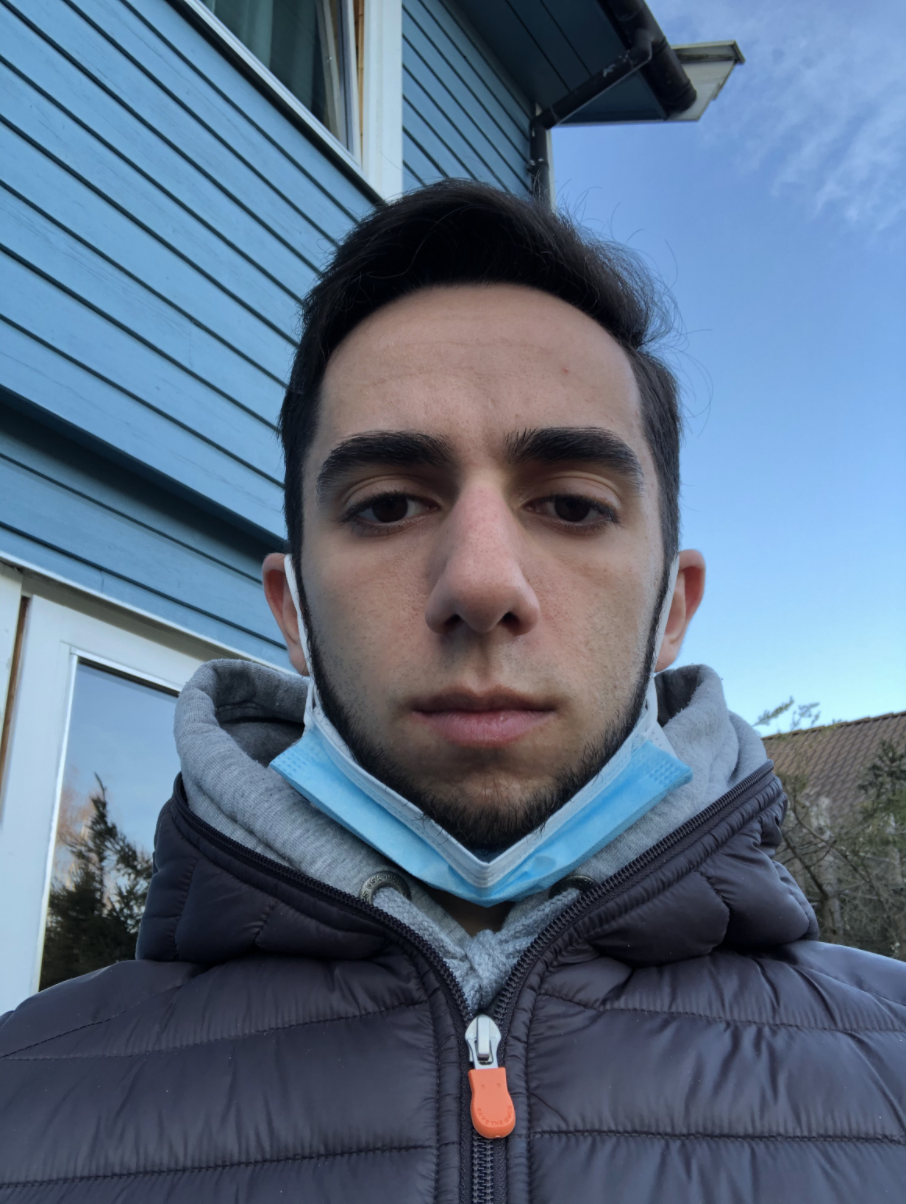
\includegraphics[scale = 0.09]{figures/926.png}\hspace{0.4cm}}
    \subfloat[0940.jpg]
        {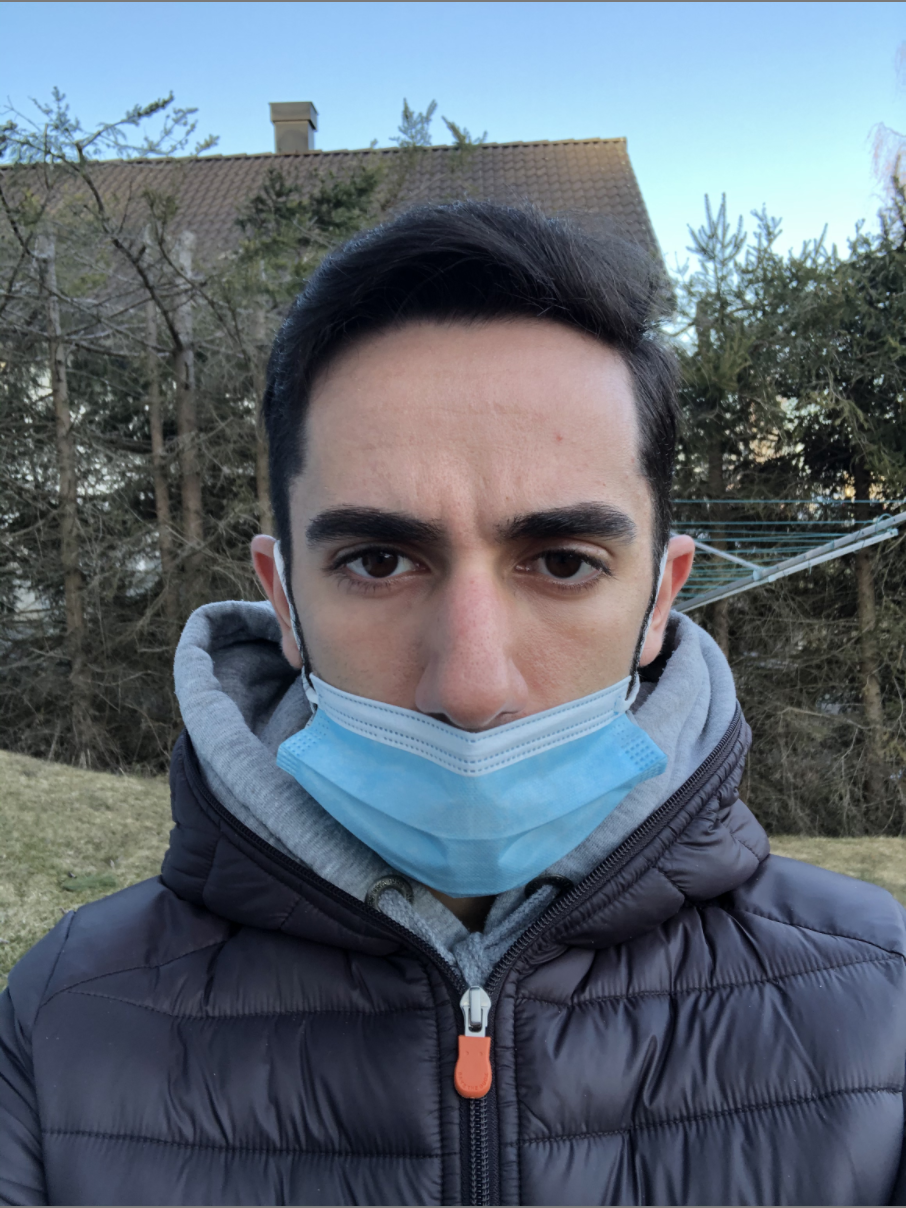
\includegraphics[scale = 0.09]{figures/940.png}\hspace{0.4cm}}
    \subfloat[1133.jpg]
        {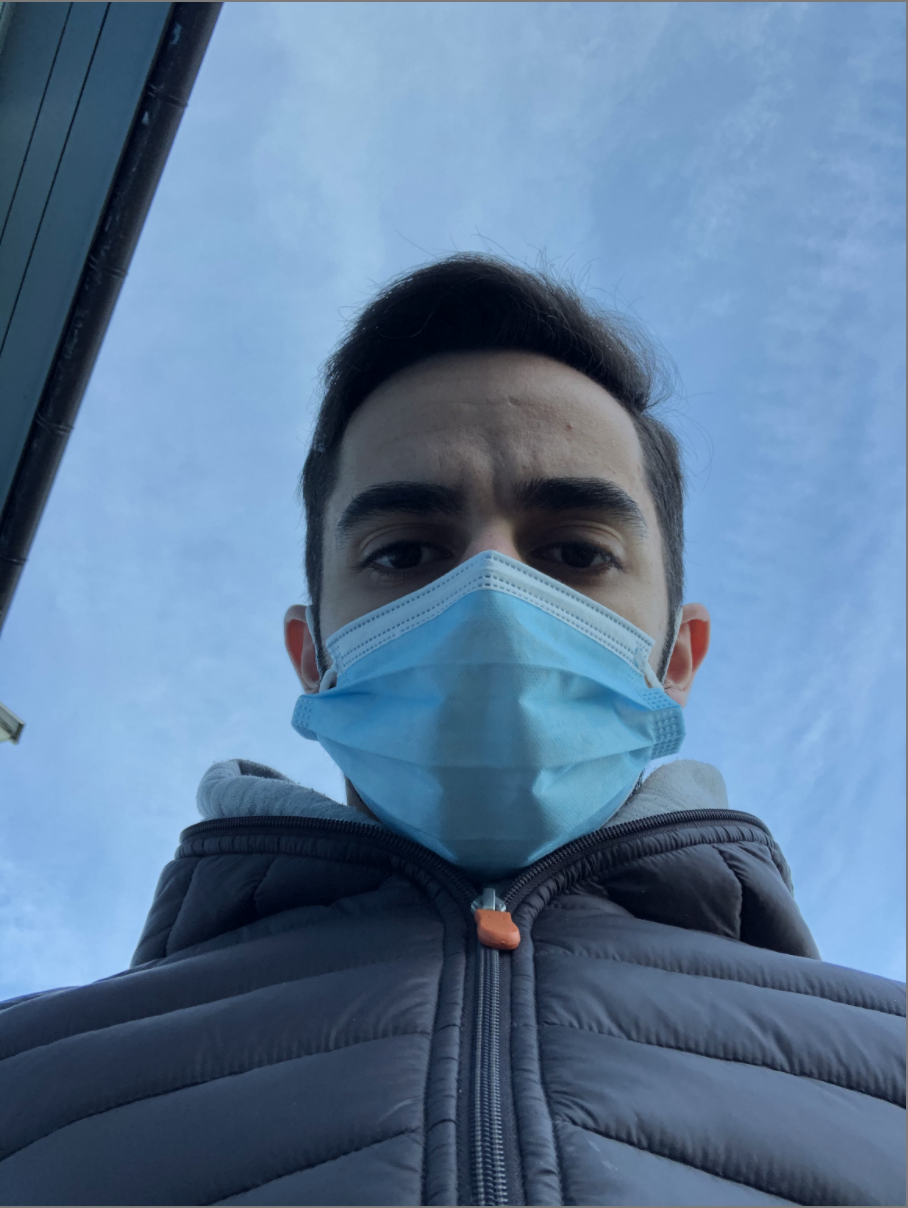
\includegraphics[scale = 0.09]{figures/1133.png}\hspace{0.4cm}}
    \subfloat[1152.jpg]
        {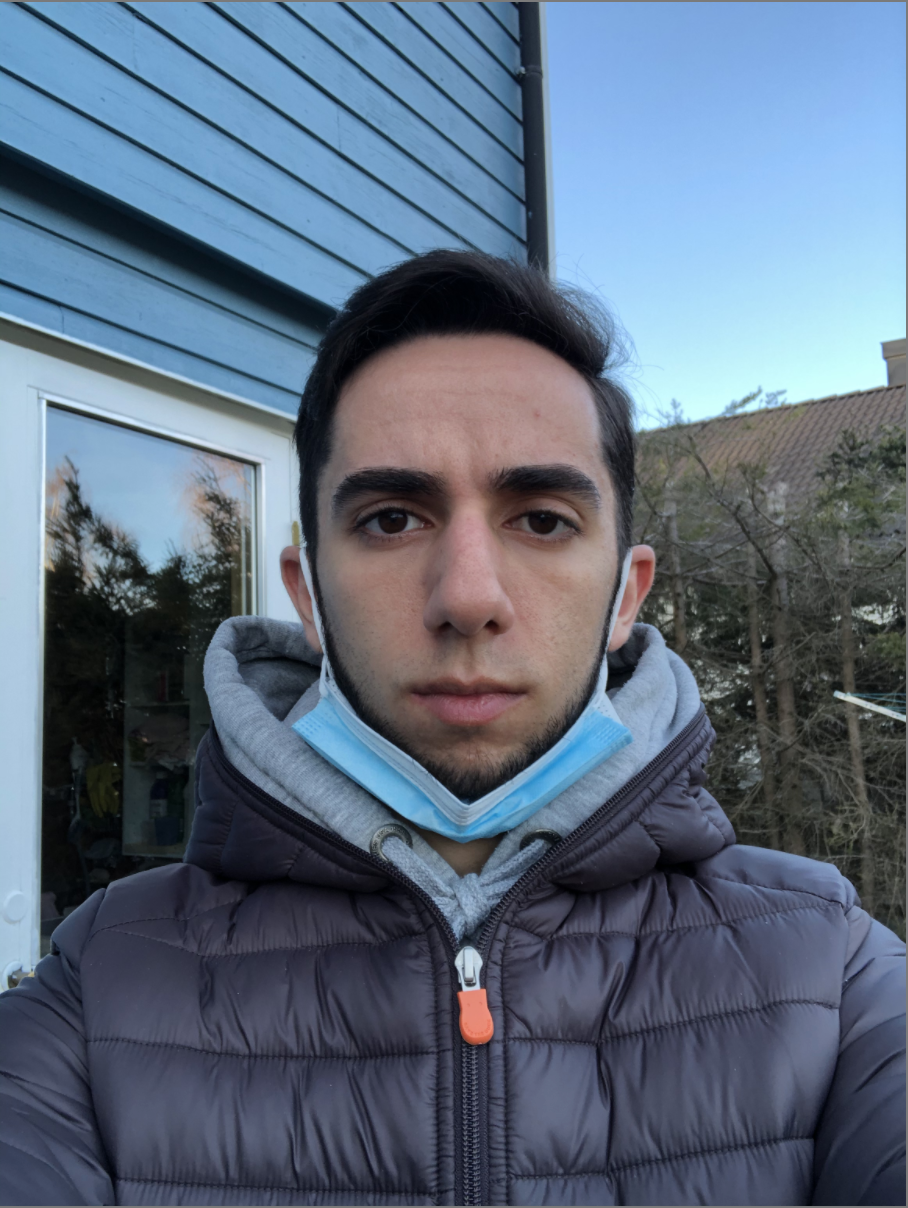
\includegraphics[scale = 0.09]{figures/1152.png}\hspace{0.4cm}}
    \caption{Spider chart of the objective and subjective scores on different face mask images.}
    \label{fig:spiderMask}
\end{figure}
\newpage

\begin{figure}[H]
\centering
    \subfloat[Different oblique angles.]
        {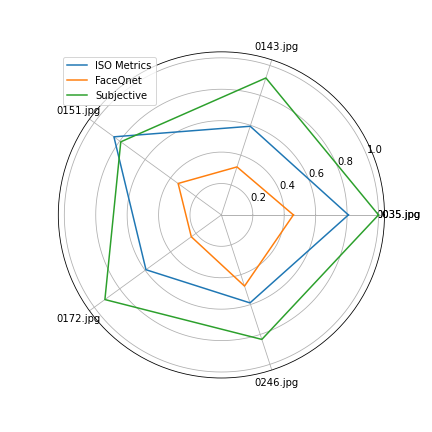
\includegraphics[width=0.4\textwidth]{figures/SpiderTilted.png}} \\
    \subfloat[0035.jpg]
        {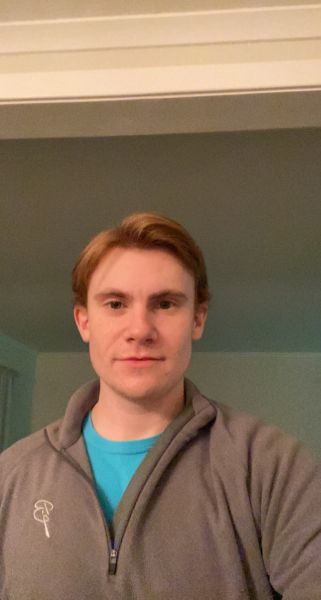
\includegraphics[scale = 0.12]{figures/0035.jpg}\hspace{0.4cm}}
    \subfloat[0143.jpg]
        {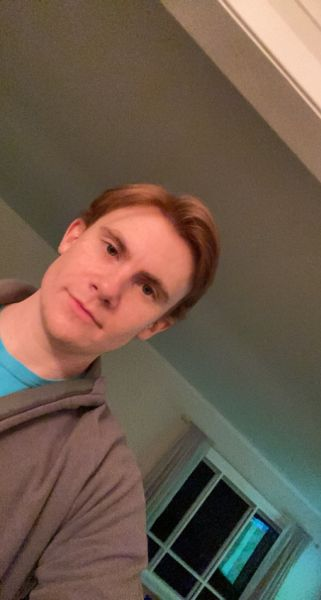
\includegraphics[scale = 0.12]{figures/0143.jpg}\hspace{0.4cm}}
    \subfloat[0151.jpg]
        {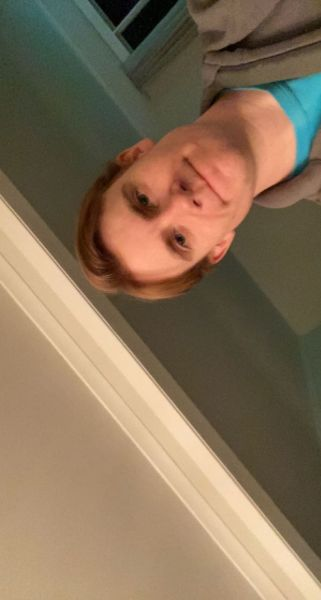
\includegraphics[scale = 0.12]{figures/0151.jpg}\hspace{0.4cm}}
    \subfloat[0151.jpg]
        {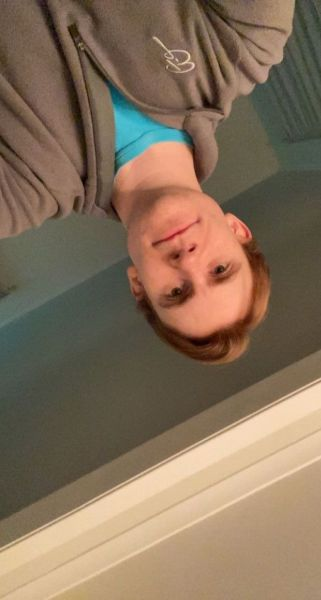
\includegraphics[scale = 0.12]{figures/0172.jpg}\hspace{0.4cm}}
    \subfloat[0246.jpg]
        {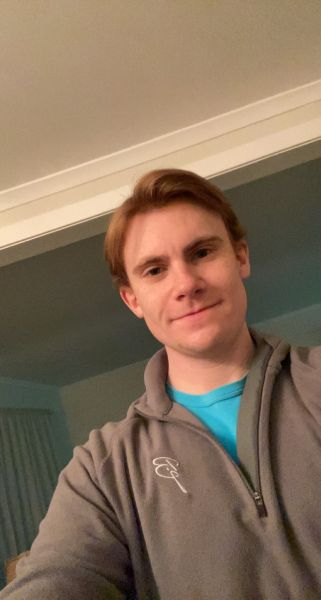
\includegraphics[scale = 0.12]{figures/0246.jpg}\hspace{0.4cm}}
    \caption{Spider chart of the objective and subjective scores on images with different oblique angles.}
    \label{fig:spiderTilted}
\end{figure}

\raggedbottom

\begin{figure}[H]
    \centering
    \subfloat[0329.jpg distorted.]
        {\includegraphics[width=0.4\textwidth]{figures/SpiderDistortions.png}} \\
    \subfloat[Original.]
        {\includegraphics[scale = 0.09]{figures/0329.jpg}\hspace{0.7cm}}
    \subfloat[Blur.]
        {\includegraphics[scale = 0.09]{figures/0329blur.jpg}\hspace{0.7cm}}
    \subfloat[Noise.]
        {\includegraphics[scale = 0.09]{figures/0329noise.jpg}\hspace{0.7cm}}
    \subfloat[Photoshop\\ compression.]
        {\includegraphics[scale = 0.09]{figures/0329photoshop_compression.jpg}\hspace{0.7cm}}
    \subfloat[Telegram\\ compression.]
        {\includegraphics[scale = 0.09]{figures/0329telegram_compression.png}\hspace{0.7cm}}
    \caption{Spider chart of the objective and subjective scores on original and distorted facial images.}
    \label{fig:SpiderDist1}
\end{figure}

\newpage

\begin{figure}[H]
\centering
    \subfloat[0718.jpg distorted.]
        {\includegraphics[width=0.42\textwidth]{figures/SpiderDistortions2.png}
        \label{fig:dist2}} \\
     \subfloat[Original.]
        {\includegraphics[scale = 0.09]{figures/0718.jpg}\hspace{0.7cm}}
    \subfloat[Blur.]
        {\includegraphics[scale = 0.09]{figures/0718blur.jpg}\hspace{0.7cm}}
    \subfloat[Noise.]
        {\includegraphics[scale = 0.09]{figures/0718noise.jpg}\hspace{0.7cm}}
    \subfloat[Photoshop\\ compression.]
        {\includegraphics[scale = 0.09]{figures/0718photoshop_compression.jpg}\hspace{0.7cm}}
    \subfloat[Telegram\\ compression.]
        {\includegraphics[scale = 0.09]{figures/0718.jpg}\hspace{0.7cm}}
    \caption{Spider chart of the objective and subjective scores on original and distorted facial images.}
    \label{fig:spiderDist2}
\end{figure}